\glsresetall
\section{Background}
\label{sec:background}

This section will highlight some important pieces of the history of past research in relevant fields.

\subsection{Computational semantics}

[semantics]
Philosophers have long been interested in the study of meaning.
Frege.
[Frege?, formal semantics, Montague ...]

A well-established and largely capable formalism for expressing and operating on propositions is first-order logic (FOL).
["classical" computational semantics]
Computational accounts of meaning emerged [how].
They are/were characterized by [what].
[Montague, ...]
[FOL/FOPC]
\citep{BlackburnComputationalsemantics2003}


[modern methodologies]
With recent advancements in computer science, ambitious computational-semantic theories are now in abundance.
As a competitor to formal systems, statistical methods have emerged which do well in various tasks within semantics.
They utilize the performance of modern computers and leverage the large amounts of data that are available as a product of our largely digitalized society.


[formal systems]
If statistical models of semantics do well in [empirical/data-driven/practical] tasks, formal theories of semantics [do what?]
\cite{BlackburnComputationalsemantics2003}:
FOPC for the win, but ``other approaches are both possible and interesting''.





\subsubsection{Perceptual semantics}
% ... in general, and spatial relations in particular

\cite{Garnhamunifiedtheorymeaning1989}:
Left/right/above/below/front/behind.
Basic meaning (of spatial relational terms).
Framework vertical constraint.
Gravitation. NESW.
Clark: canonical encounter? (left of cabinet, left of chair.)
(Ships and outer space.)

\cite{LoganComputationalAnalysisApprehension1996} account for the state of 
Basic–deictic(–intrinsic) relations.
Perceptual–conceptual representation.
"Computational theory of apprehension": spatial indexing -> reference frame -> ... Instead, we move into the conceptual level, both in perception and language, and evaluate validity from there.
(Drawbacks?)
They present "evidence" for their theory, does that evidence contradict the present approach?

lo, refo? (refo used bleow)

Terms of spatial relations (\textit{behind}, \textit{to the left of}, etc.) have three types of meanings \citep{Garnhamunifiedtheorymeaning1989}: basic, deictic and intrinsical.
The deictic and intrinsical meanings hold for relations between two objects.
The deictic meaning is relative to the coordinate frame of the speaker, while the intrinsical is relative to that of the reference object.
The basic meaning, introduced by \cite{Garnhamunifiedtheorymeaning1989}, is also relative to the speaker, but holds for a single object only.
[and? (it is basic in the way that... what?) example?]

\cite{RegierGroundingspatiallanguage2001a}:
Four models. AVS.
Many experiments.
Spatial term ratings influenced by: proximal \& center-of-mass orientations, grazing line, distance.

\cite{CoventryClassificationExtrageometricInfluences2004}:
Extra-geometric constraints on the meaning of spatial relational terms.
Especially functional.
Functional geometric framework.
[functional aspect, Coventry?]

\cite{HarnadSymbolGroundingProblem1990}:
Can a computer really ``understand'' concepts, that is, will it operate on grounded symbols or just the (arbitrary) symbols themselves?
Turing test.

\cite{SteelsSymbolGroundingProblem2007}:
Peirce: object, symbol, concept. Grounded with method.
Searle and other claim that the Symbol grounding problem is insolvable.
Steels concludes that it is solved.
Using experiments where a number of agents participate in a language game where they make up random words for preset concepts and manage to ``agree'' on which words to use for which concepts.

...



\subsection{Type theory in natural language processing}

Type theory was developed as an alternative to set theory, responding to paradoxes found in the latter.
With set theory widely serving as a \textit{foundation of mathematics}, the development of this new theory was [important].
Several different type theories have been created, of which Church's \textit{simply typed \textlambda-calculus} \cite{church40} and Martin-Löf's \textit{intuitionistic type theory} \citep{martinlof84} are some prominent examples.
\citep{CoquandTypeTheory2015} [too detailed?]

[use of type theory in nlp]

\cite{CooperRecordsRecordTypes2005} combines several theories from logic, semantics and linguistics in a single framework called \textbf{\acrfull{ttr}}.
 lambda calculus, phrase structure grammar, (DRT), (situation semantics) (what are the latter)?
It has been employed to model natural language in the context of dialogue, situated agents and spoken language.

[brief summary of TTR syntax?]



\subsubsection{Perceptual semantics in \gls{ttr}}

\cite{LarssonDialoguesHaveContent2011}

\cite{DobnikModellinglanguageaction2012}

\cite{lspc} model the point space perception of a mobile robot equipped with a rangefinder.
 that would move around and use laser range scanner or similar to collect points in space, group them into objects and detect spatial relations between them.
\Gls{ttr} is mainly used to model the transition from the perceptual to the cognitive domain as well as 
 throughout the model, accounting for perception and cognition.

\cite{ttrspat} develop this further, focusing especially on spatial relations.

\cite{LarssonFormalsemanticsperceptual2015}

Parsing: \cite{CooperRecordsRecordTypes2005}, \cite{RobinCooperAustiniantruthattitudes2005}, \cite{CooperTypetheorysemantics2012}, \cite{CooperTypetheorylanguage2016}



\subsubsection{PyTTR}

\cite{pyttr} is a Python implementation of \gls{ttr}.
It supports modeling records, record types, ptypes, functions and other TTR objects.
Additionally, it allows operations such as judgement, type checking and subtype checking.
As a Python library it also enables other features and peripheral procedures to be written in Python.

[the advantage of implementing a theoretical model]
PyTTR, itself being an implementation of TTR, allows, in turn, the implementation of models and theories that build on TTR.
By implementing a theoretical model as a computer program, it can ``come alive'' and be tested on real problems and data.
Another motivation for implementation is to compete with existing, less theoretically strong techniques to solve a given task, but it is possibly secondary to the former reason.

%[What has been written in PyTTR so far? nu, animat]



\subsection{Computer vision}

[computer vision]

[object recognition]

You only look once (YOLO) \citep{RedmonYouOnlyLook2015} is a neural network model that simultaneously predicts bounding boxes around objects and classifies the contained objects.

Among the most recent contributions to computer vision, Facebook's \textit{Detectron} \citep{Detectron2018} features outlining of identified objects and classification with impressive accuracy.

\begin{figure}[h]
\label{fig:dogbike_annotated}
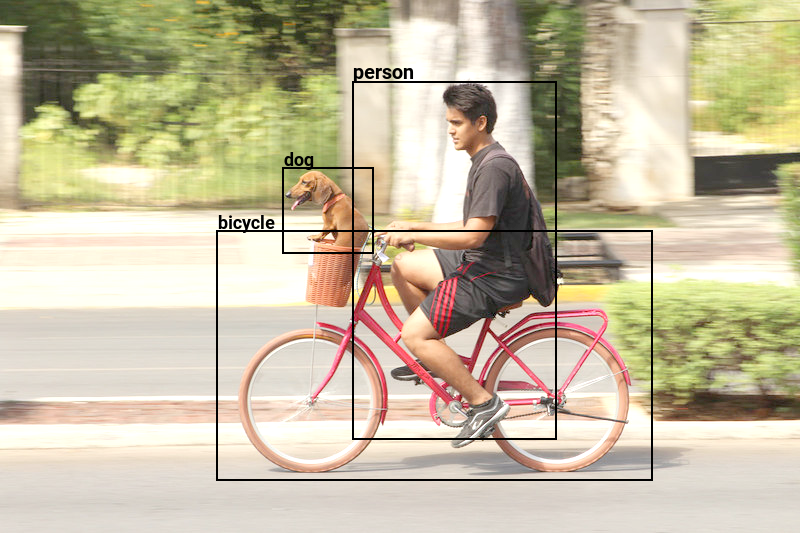
\includegraphics[width=\textwidth]{dogbike_annotated}
\centering
\caption{Visualization of the labels and bounding boxes emitted by YOLO when given an image depicting a cyclist with a dog.}
\end{figure}



\subsubsection{\Acrfull{vqa}}

\cite{AgrawalVQAVisualQuestion2015} suggest \acrfull{vqa} as a [complete] challenge in AI-completeness.
``A VQA system takes as input an image and a free-form, open-ended, natural-language question about the image and produces a natural-language answer as the output''.
The initiative includes a dataset and a series of annual competitions since 2016.

\cite{AndreasLearningComposeNeural2016}